\section{Implementering av ny løsning}
Konstruksjonen har blitt laget og testet. I dette kapittelet vises bilder av den endelige rammekonstruksjonen samt data fra testing av rammen. 
Testingen ble i hovedsak utført ved å legge last på rammen. Det er i utgangspunktet vanskelig å beregne makslast på gammelt treverk. Dette på grunn av at det er vanskelig å anslå hvor skadet treverket er. Det er observert mange hull og skader i treverket på grunn av tidligere montering og bruk. Dette i kombinasjon med usikkerheten rundt fukt og hvor nedbrutt treverket er, gjør dimensjonering og fastsettelse av styrkeegenskaper vanskelig.
Testingen ble som nevnt utført ved å laste rammen så mye som det var forsvarlig ut ifra et subjektivt synspunkt. Det ble under testing lastet i overkant av 200 kg på rammen. Dette blir derfor anbefalt makslast på rammen. Videre er det av rammens dimensjoner gitt en maksimal lastlengde 3000 mm, en maksimal lastebredde på 1500 mm samt en maksimal lastehøyde på 1300 mm.
Bildene fra den endelige konstruksjonen er vist under.     
\begin{figure}[H]
\centering   
\subfloat[Rammen]{\includegraphics[width=0.5\textwidth]{images/NL1.JPG}}
\subfloat[Rammen på støtteben]{\includegraphics[width=0.5\textwidth]{images/NL2.JPG}}
\caption{Konstruksjonen}
\label{B1}
\end{figure}
\begin{figure}[H]
\centering   
\subfloat[Bakre låsing]{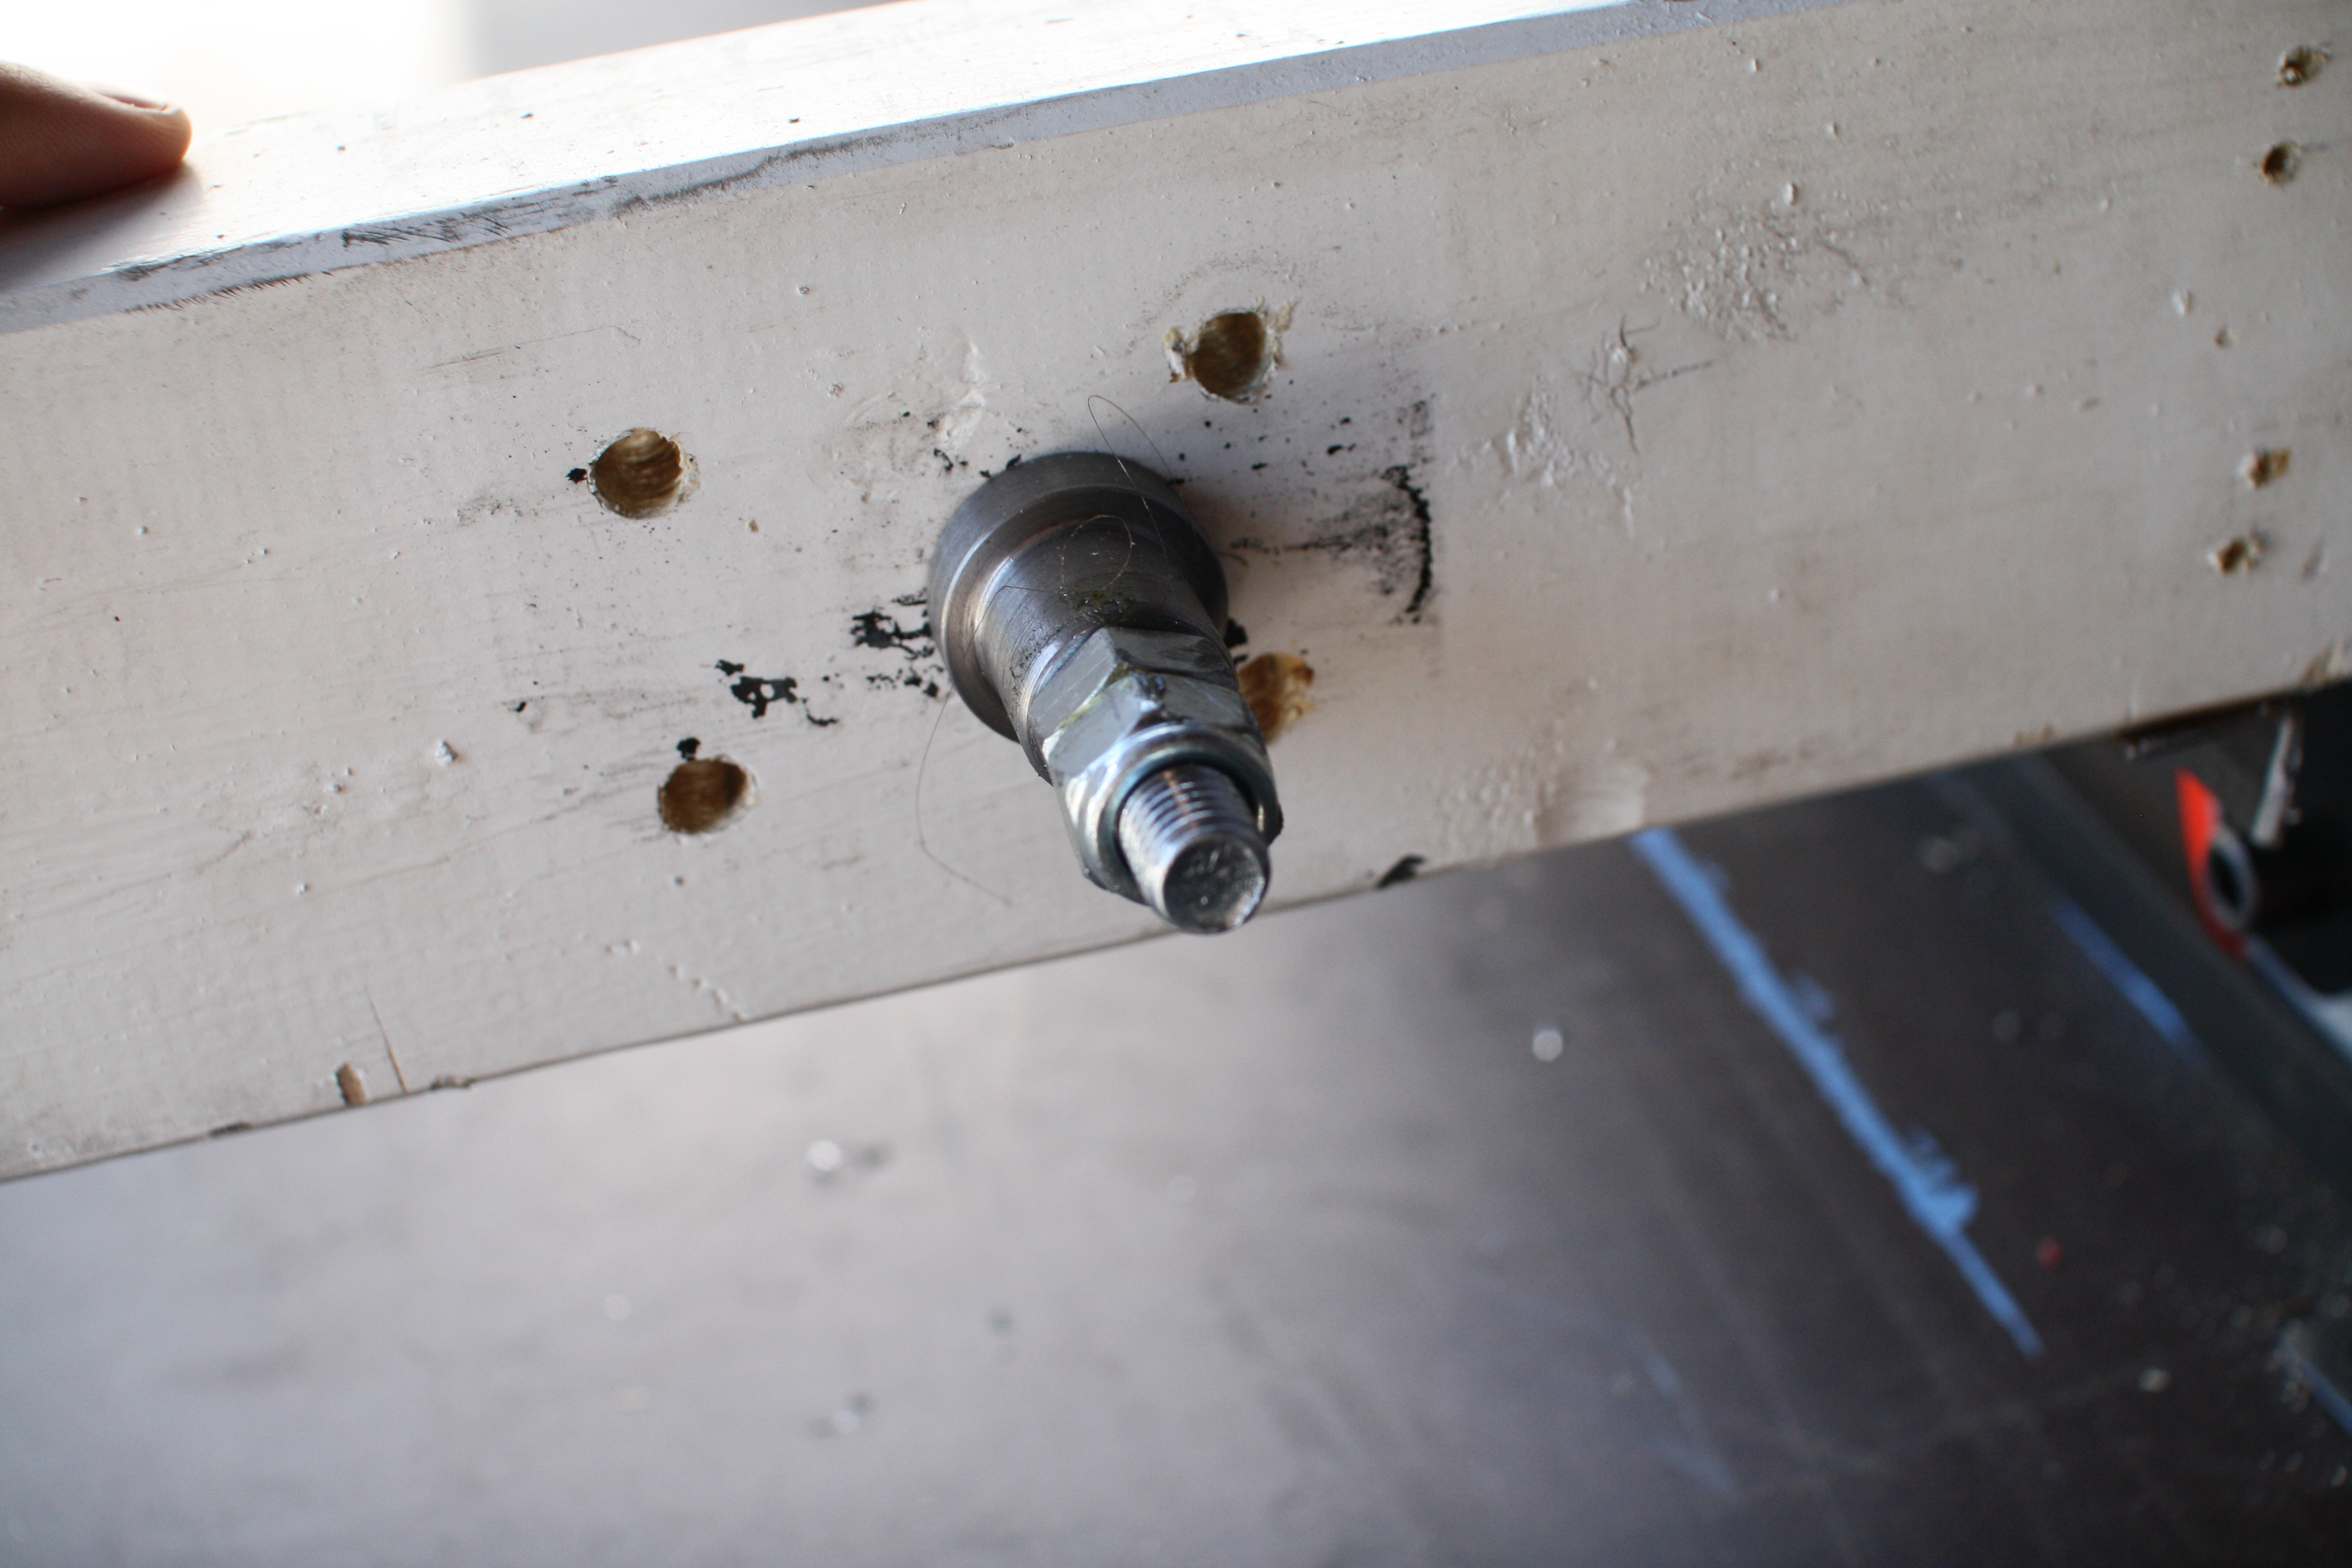
\includegraphics[width=0.45\textwidth]{images/NL3.JPG}}
\subfloat[Bakre låsetapp]{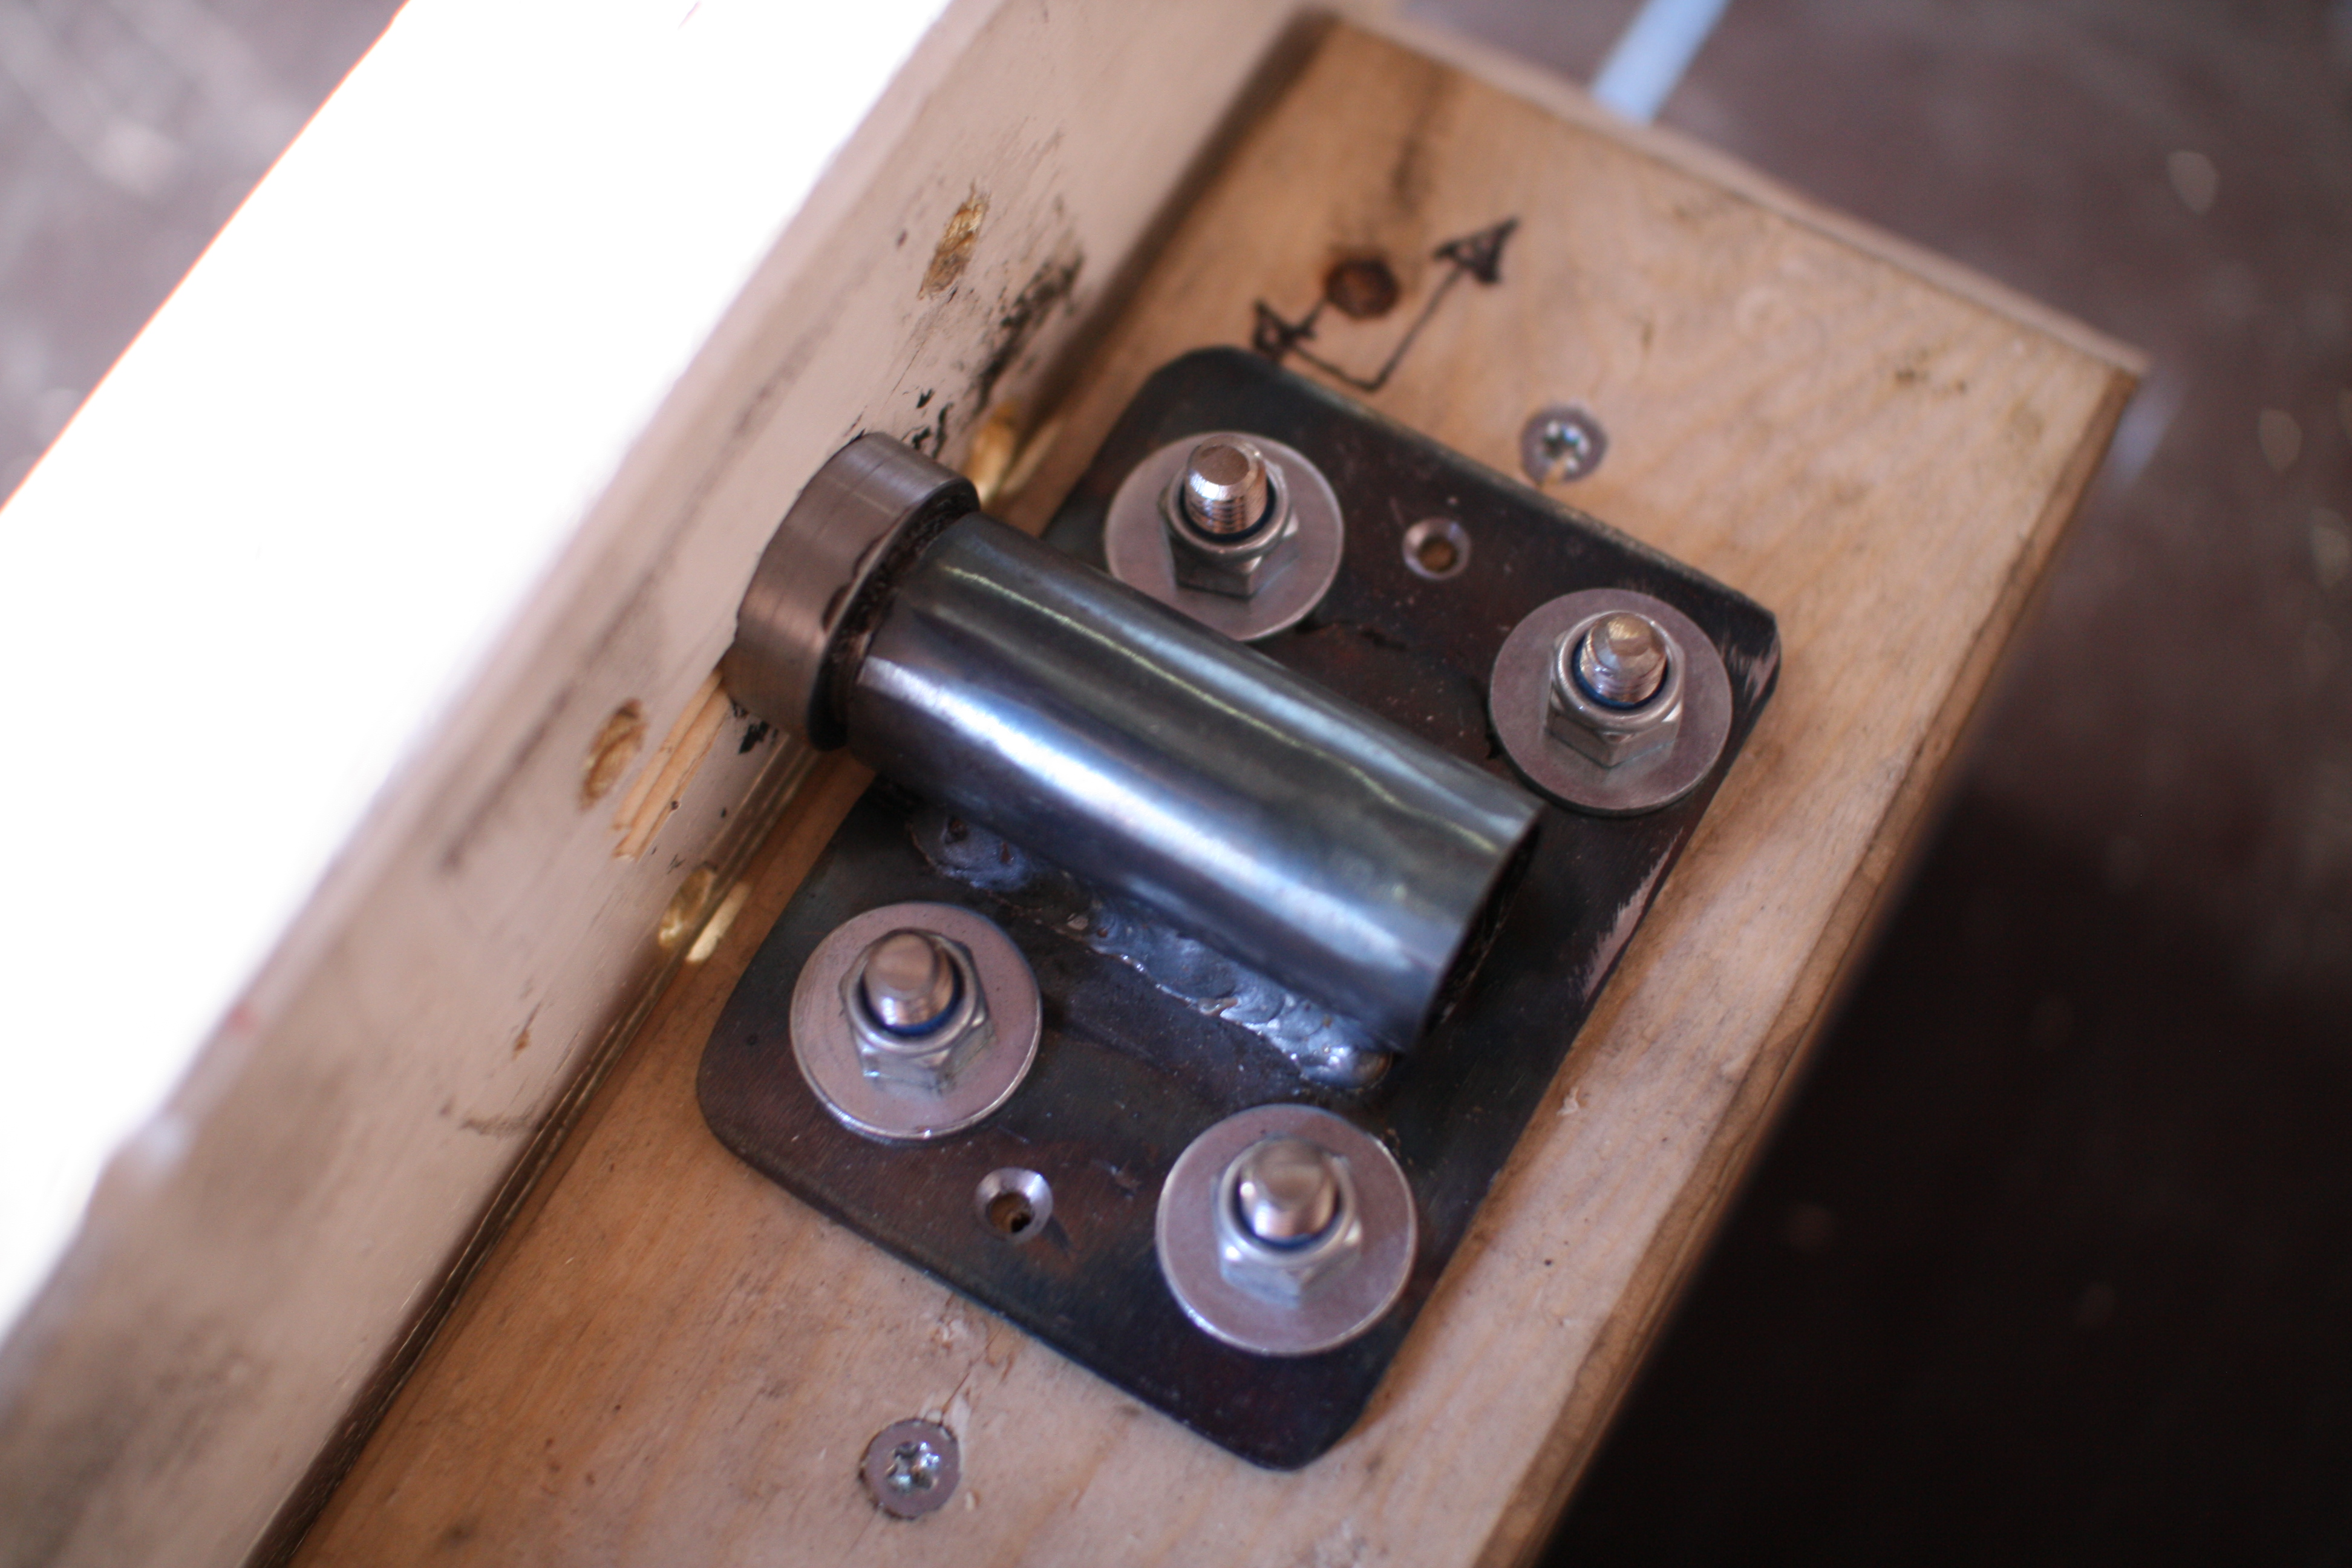
\includegraphics[width=0.45\textwidth]{images/NL4.JPG}}
\caption{Bakre låsing}
\label{B2}
\end{figure}
\begin{figure}[H]
\centering   
\subfloat[Støttebrakett]{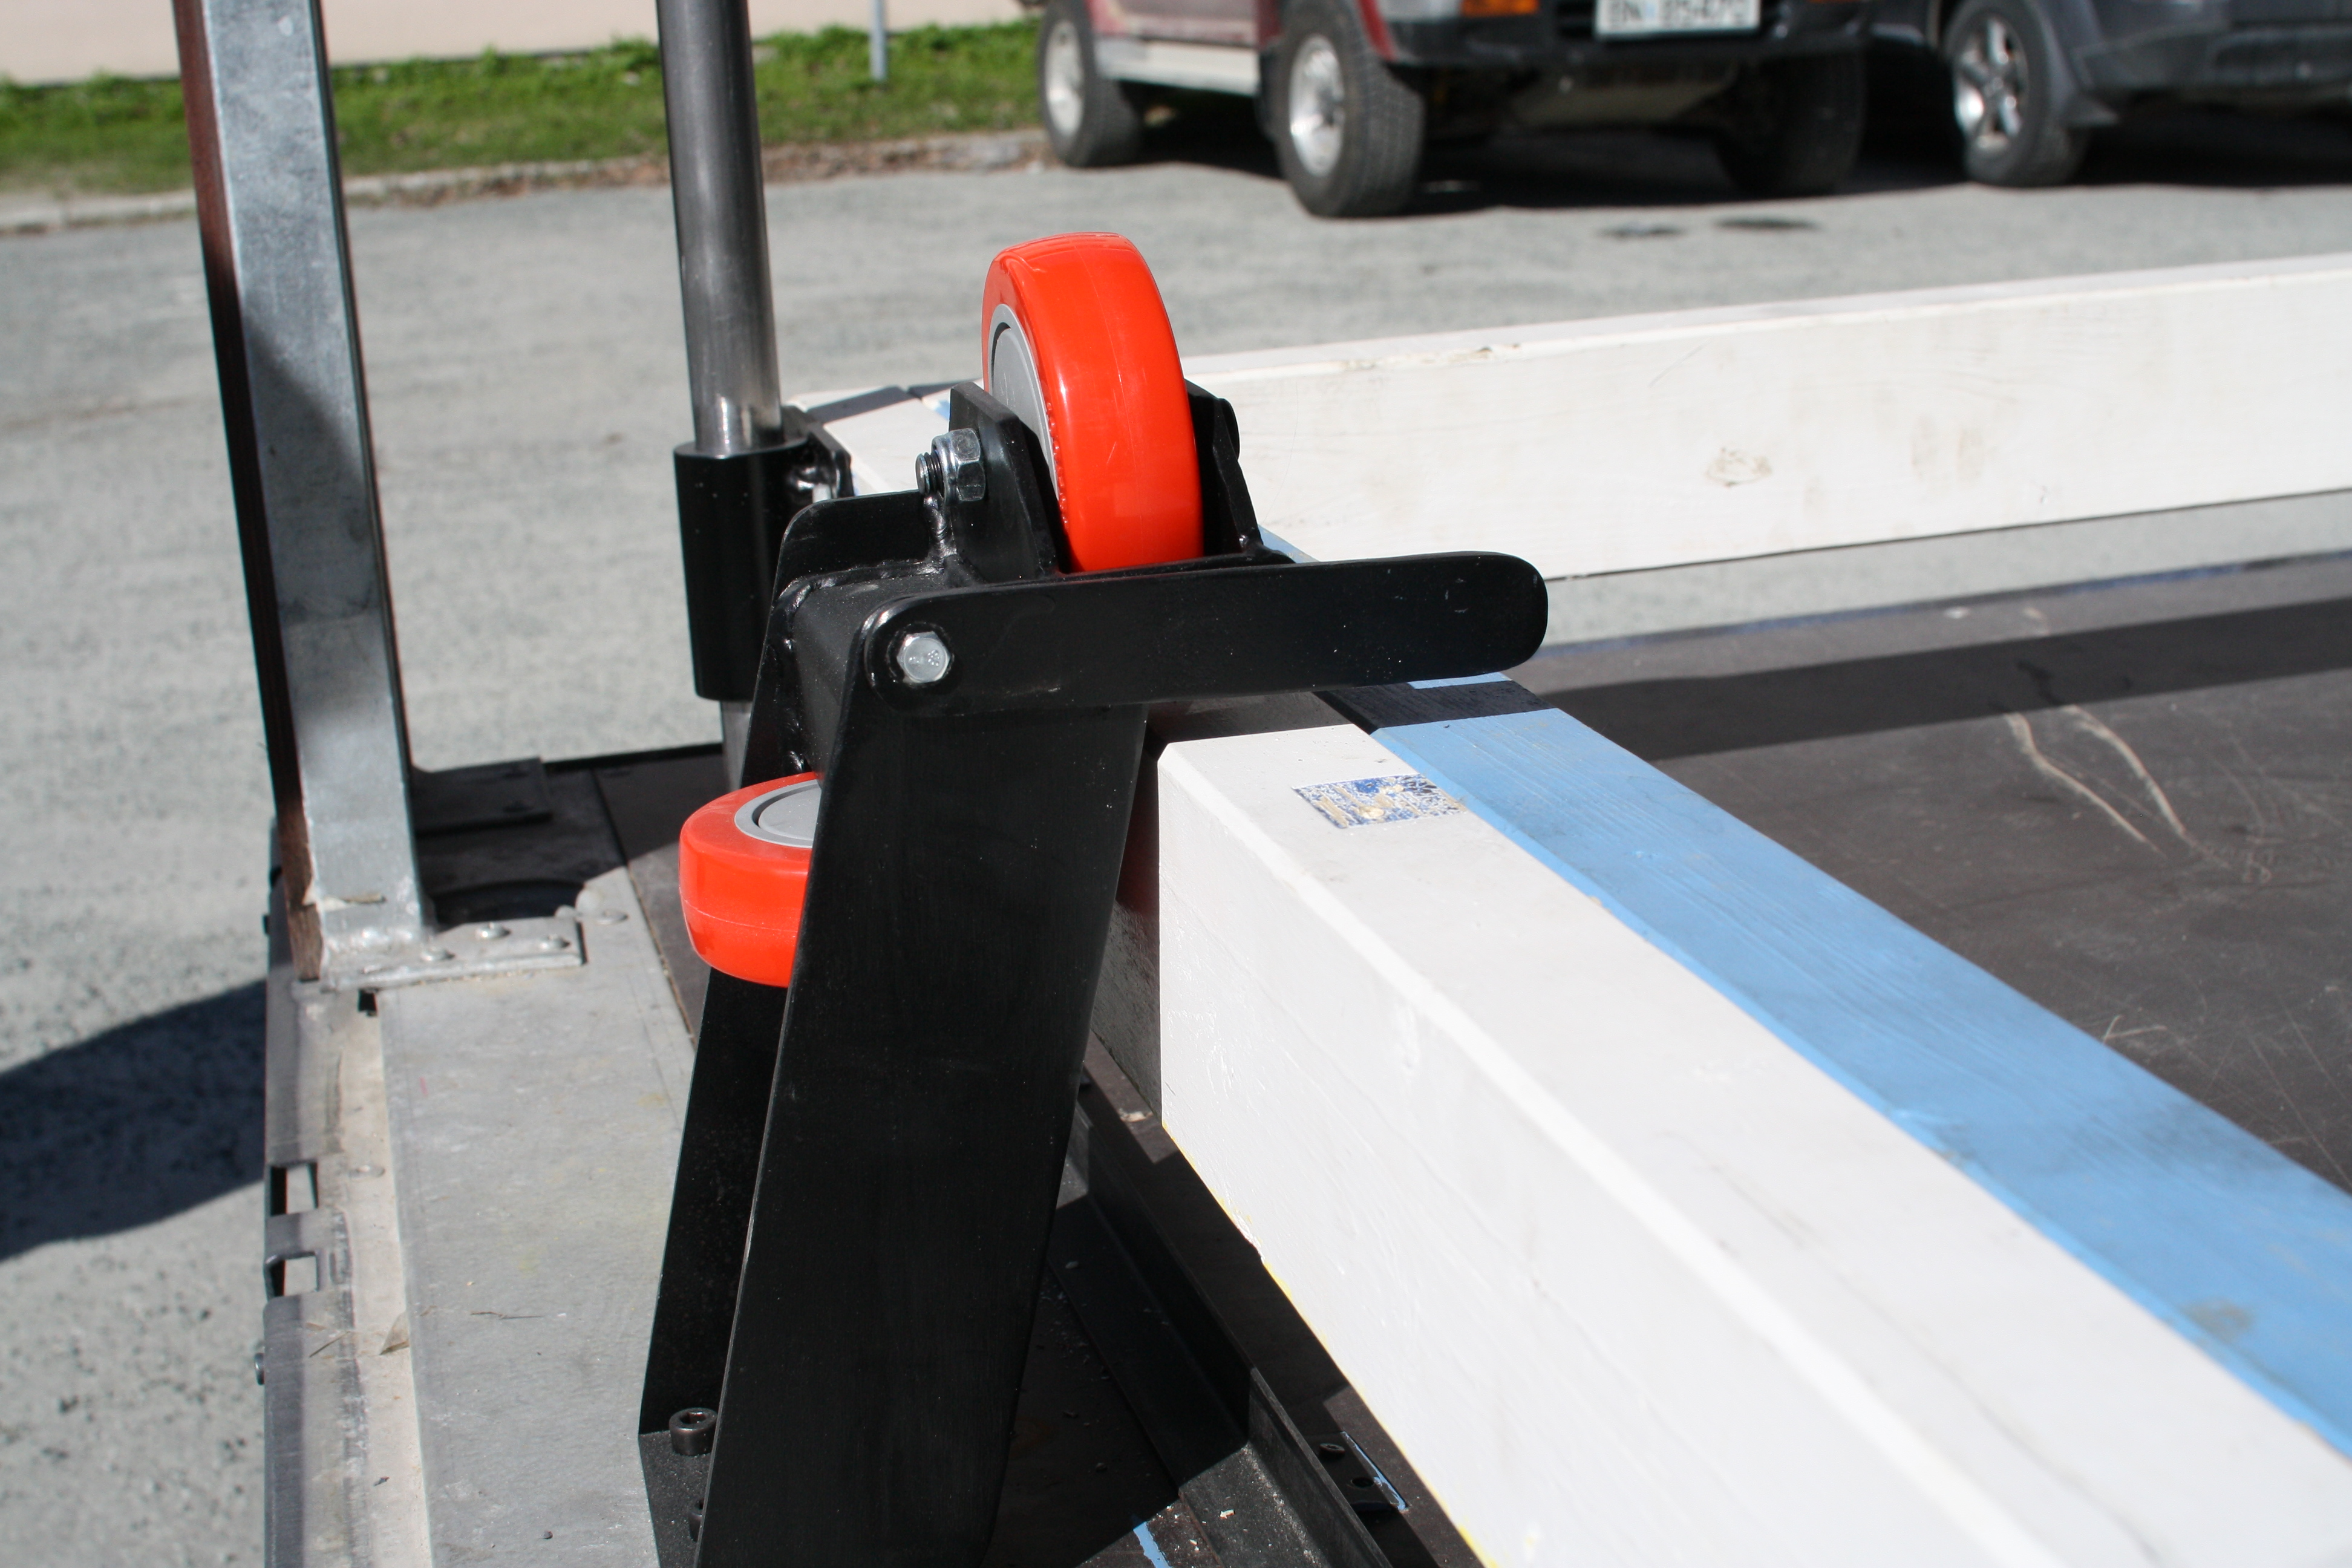
\includegraphics[width=0.45\textwidth]{images/NL5.JPG}}
\subfloat[Idiotsikring]{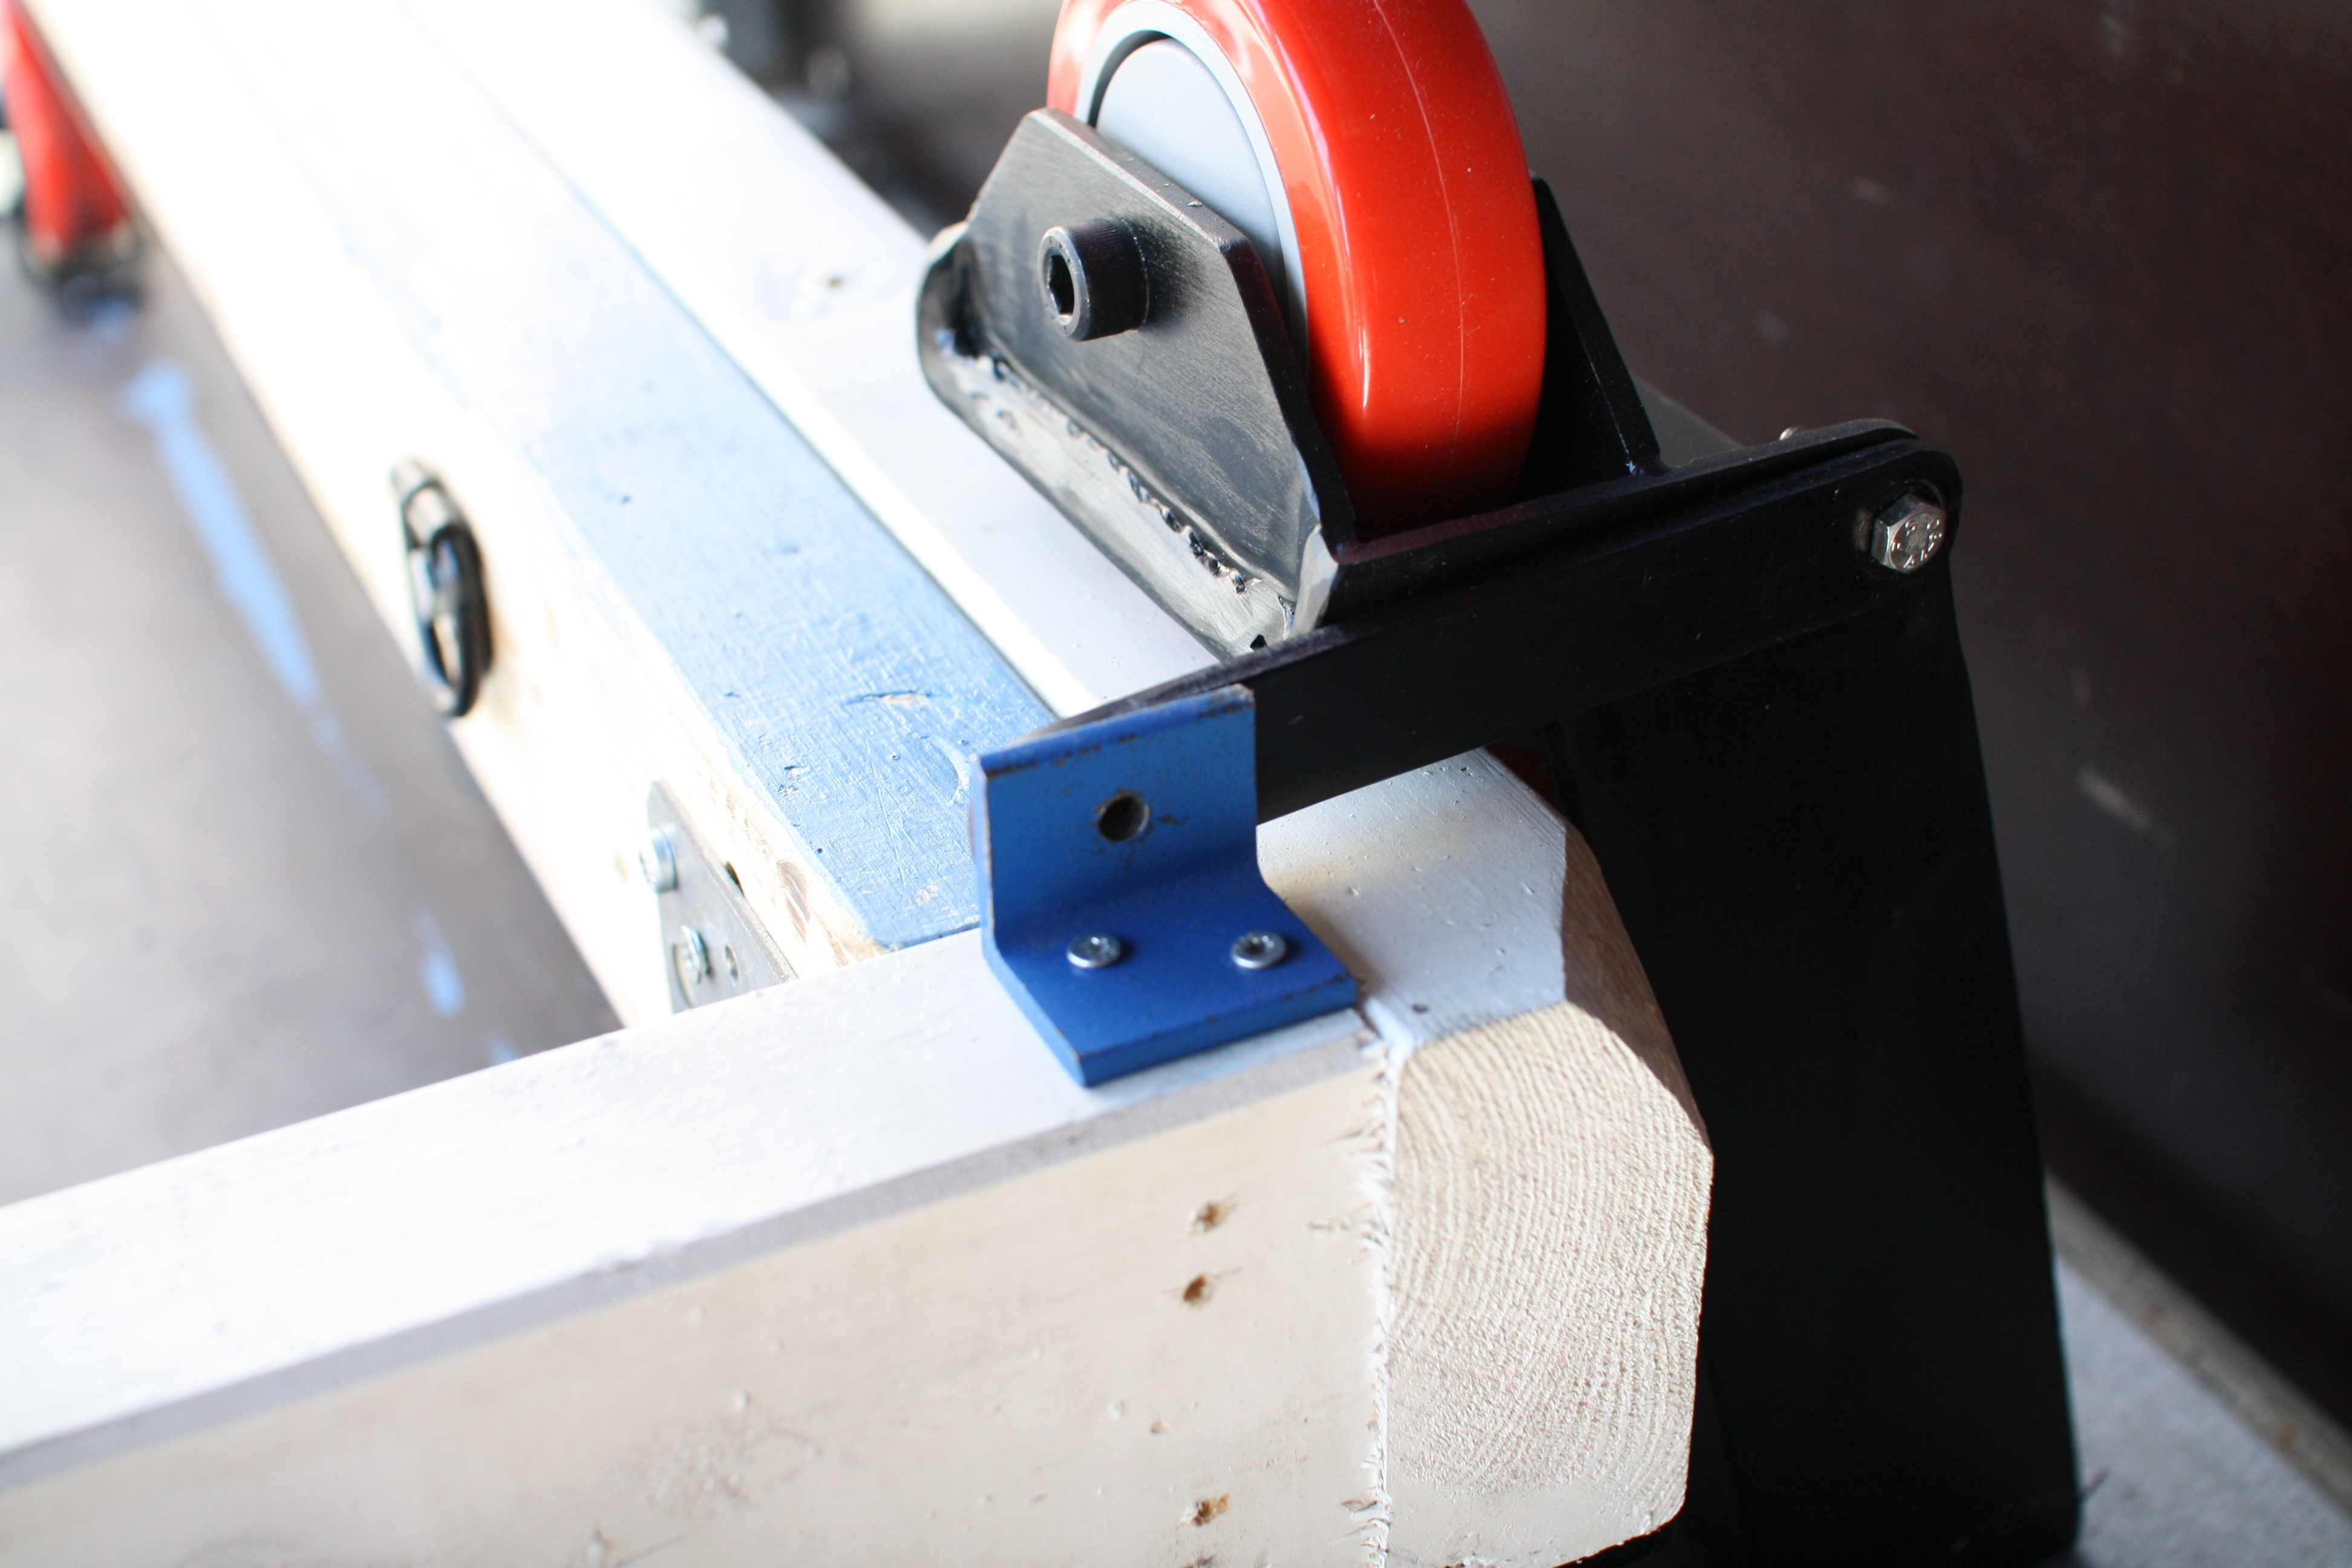
\includegraphics[width=0.45\textwidth]{images/NL6.JPG}}
\caption{Støttebrakett med sikring}
\label{B3}
\end{figure}
\begin{figure}[H]
\centering   
\subfloat[Fremre låsetapp]{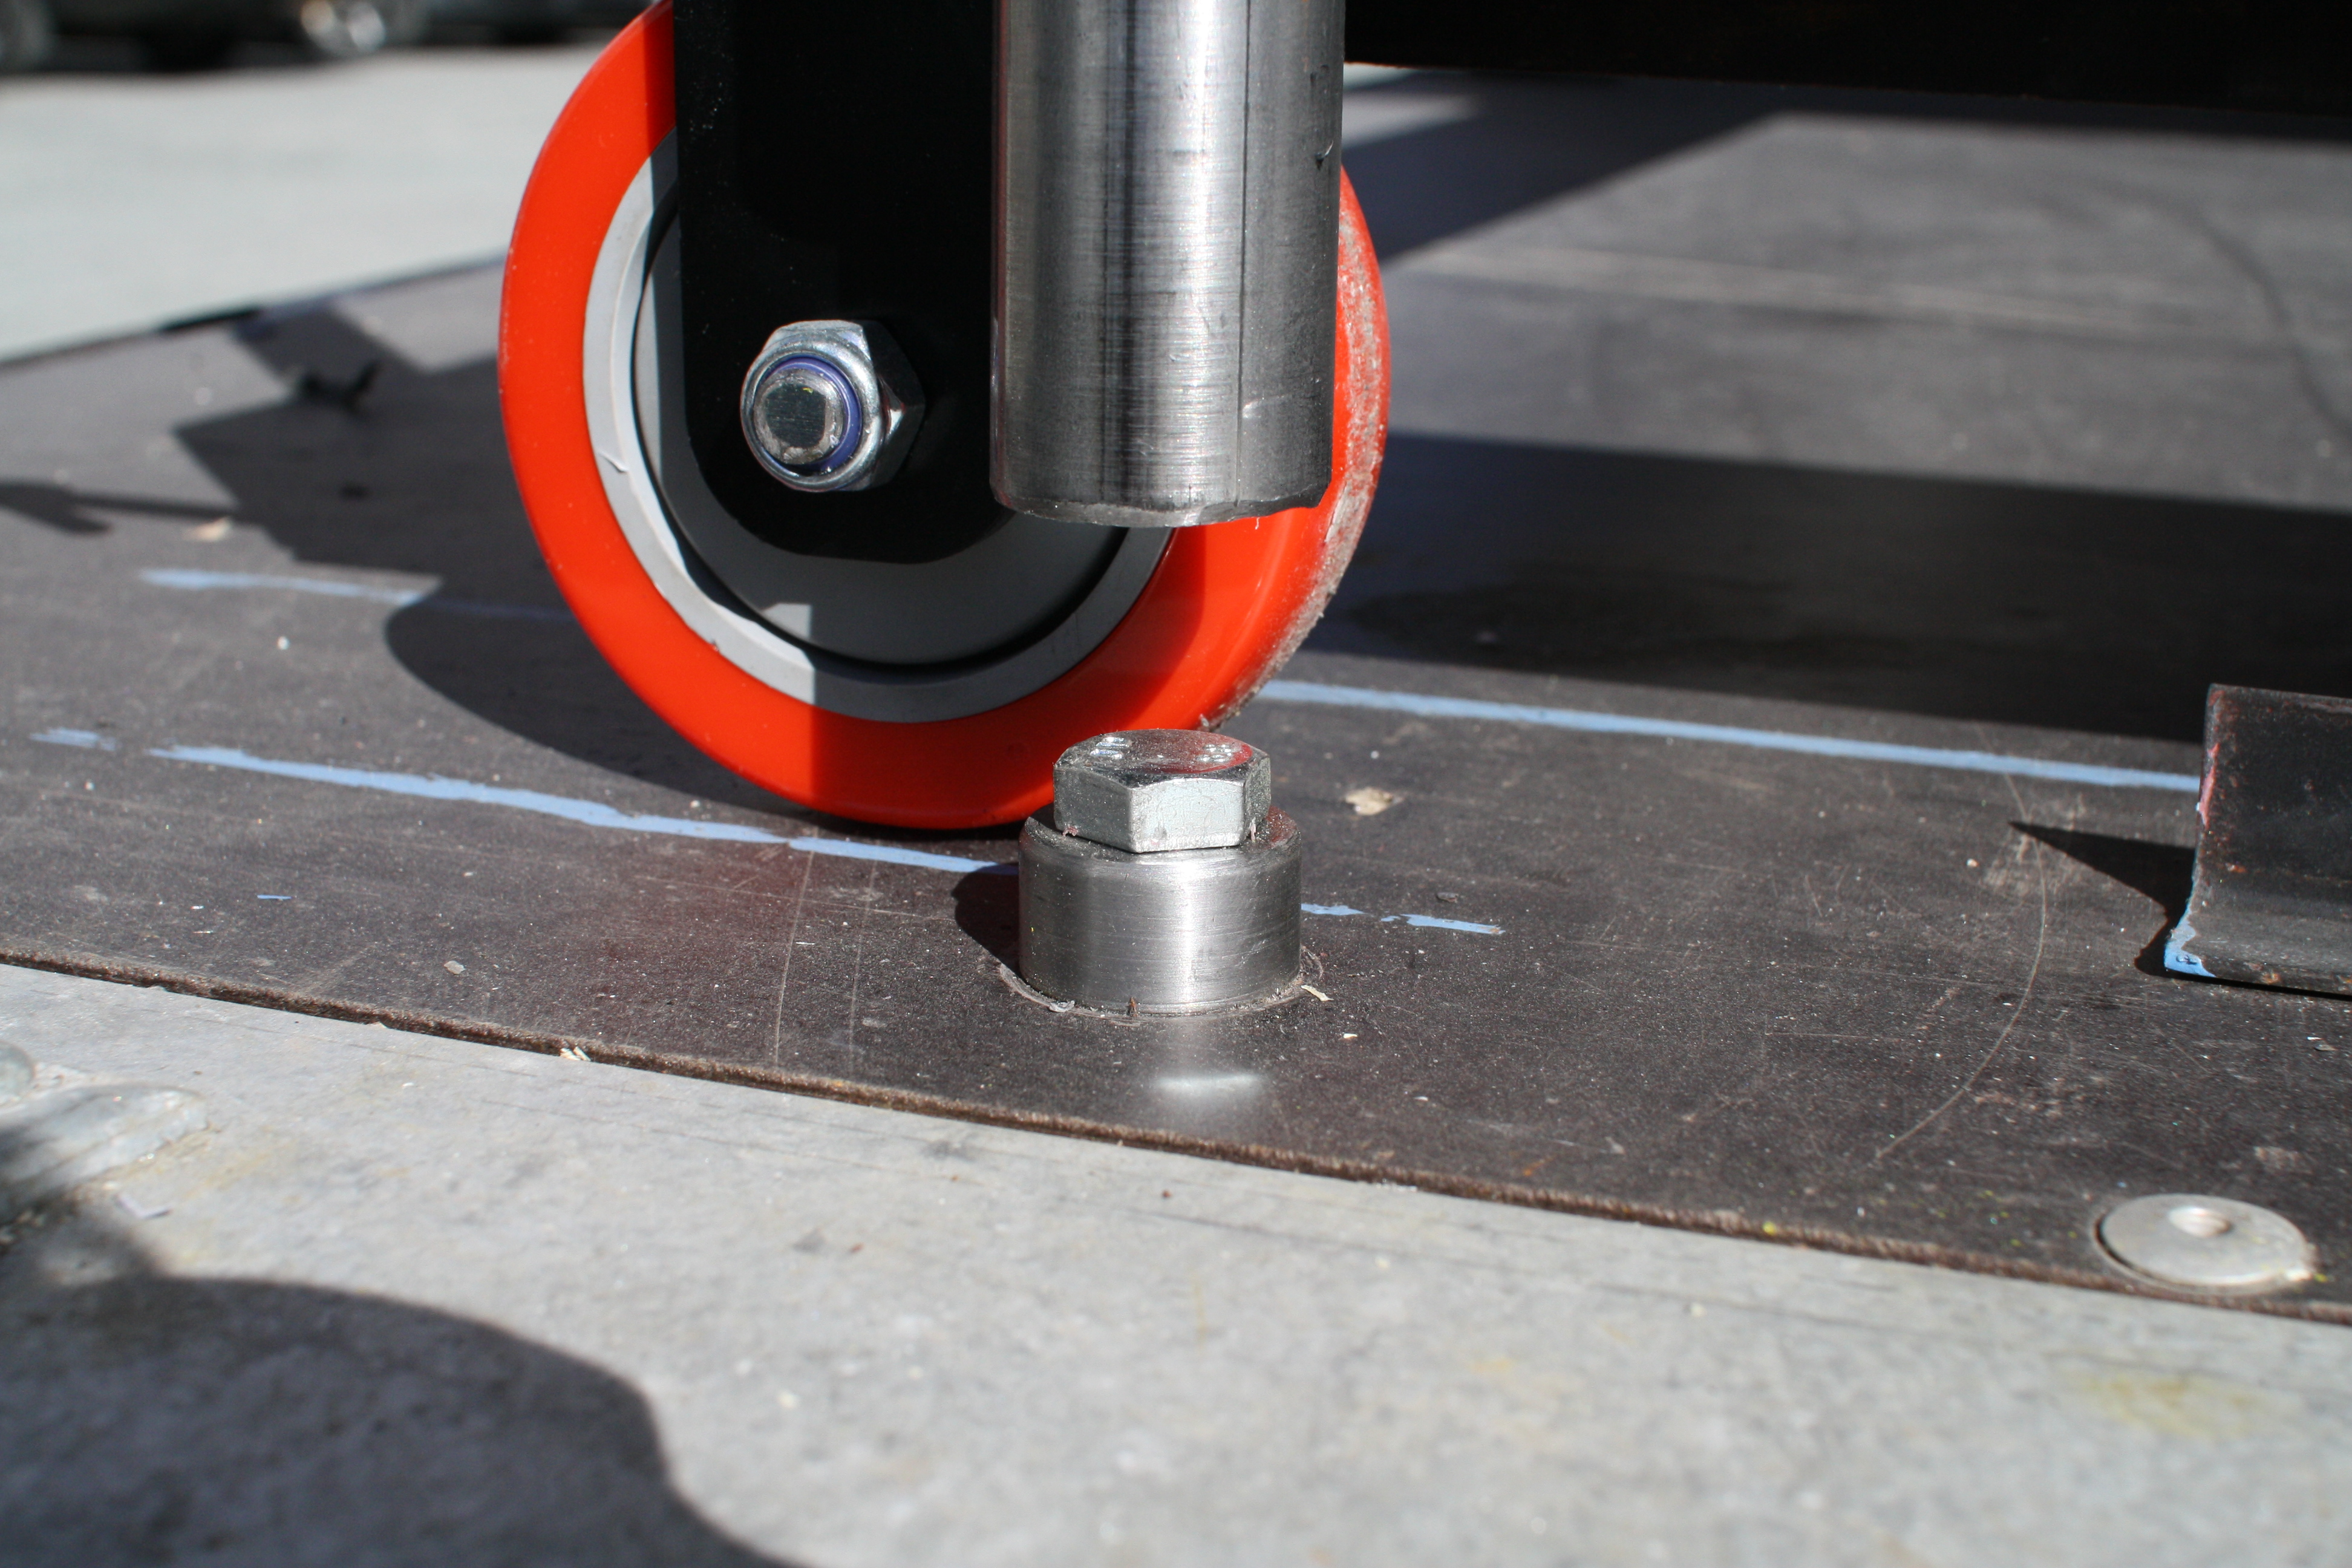
\includegraphics[width=0.45\textwidth]{images/NL7.JPG}}
\subfloat[Fremre låsing]{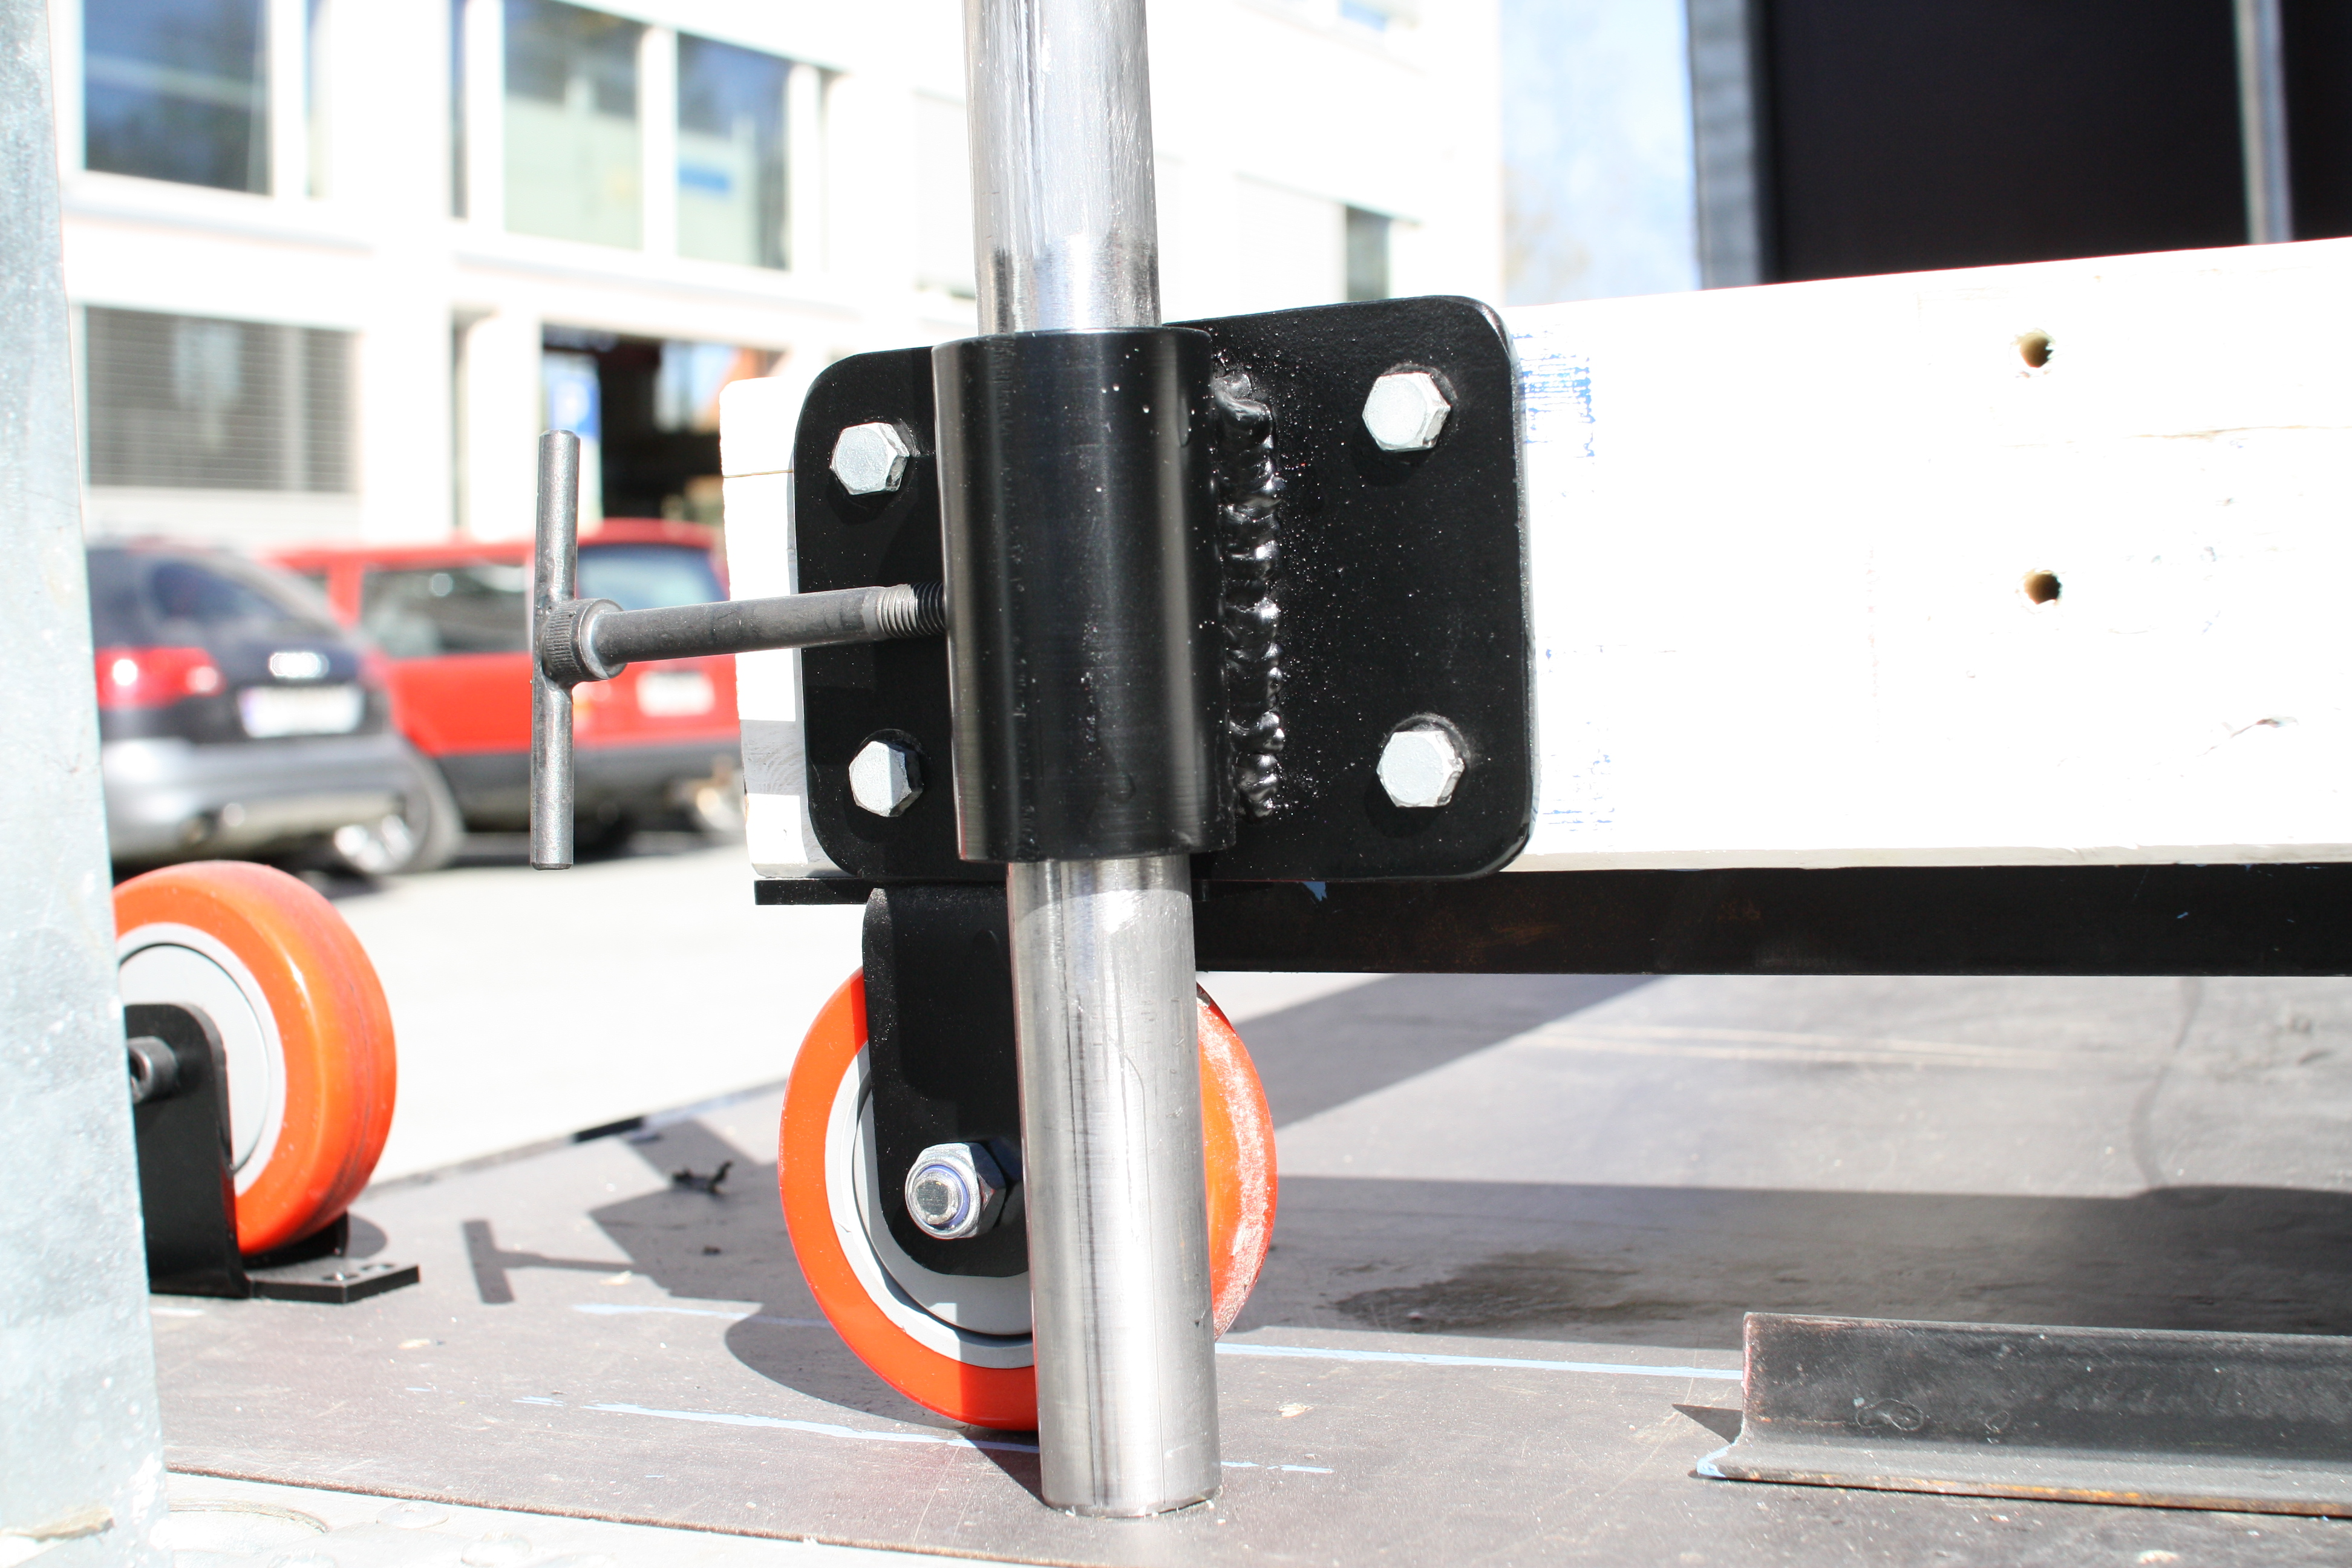
\includegraphics[width=0.45\textwidth]{images/NL8.JPG}}
\caption{Fremre låsing}
\label{B4}
\end{figure}
Figur \ref{B1} viser et oversiktsbilde av hele hengeren samt rammen når den er dratt ut og står på støttebena.
Videre i Figur \ref{B2} vises den bakre låsingen og låsetappen som skal treffe låsehylsen montert i henger når rammen blir dyttet inn. I Figur \ref{B3} vises støttebrakettene med en sikring. Denne sikringen ble ikke tatt med når konseptet ble designet, men kom som et ønske fra Shell Eco Maraton teamet under montering av systemet. 
Figur \ref{B4} viser den fremre låsmekanismen og den gjennomgående låsetappen montert i henger
\section{Budsjett og Regnskap}
Under vises i Tabell \ref{TBL1} hvilke budsjetterte utgifter som er beregnet.
\begin{table}[H]
\begin{tabular}{l l l l l}
 \textbf{Item} & \textbf{Beskrivelse} & \textbf{Antall} & \textbf{Pris} & \textbf{Totalt}  \\
\hline
001&Hovedplate&2&250.0 kr&500.0 kr\\
002&Trekantavstiver&8&62.5 kr&500.0 kr\\
003&Hjulbrakett&8&187.5 kr& 1500.0 kr\\
006&Toppavstiver&4&50.0 kr& 200.0 kr\\
007&Horisontal hjulplate&4&62.5 kr& 250.0 kr\\
-&Hjul&12&44.9 kr& 538.8 kr\\
\hline
\textbf{Sum}&&&&3488.8 kr\\
\hline
\end{tabular}
\caption{Budsjett}
\label{TBL1}
\end{table}
Videre vises i Tabell \ref{TBL2} de reelle utgiftene relatert til prosjektet. Det ble brukt 347,- mer enn budsjettert. Fremdeles er budsjettet på 5000 kr overholdt med god margin.
\begin{table}[H]
\begin{tabular}{l l l l l}
 \textbf{Item} & \textbf{Beskrivelse} & \textbf{Antall} & \textbf{Pris} & \textbf{Totalt}  \\
\hline
001&Hovedplate&2&250.0 kr&500.0 kr\\
002&Trekantavstiver&8&62.5 kr&500.0 kr\\
003&Hjulbrakett&8&187.5 kr& 1500.0 kr\\
006&Toppavstiver&4&50.0 kr& 200.0 kr\\
007&Horisontal hjulplate&4&62.5 kr& 250.0 kr\\
-&Fakturagebyr&1&50.0 kr&50.0 kr\\
-&Lakk&2&59.9 kr&119.8 kr\\
-&Hjul&12&44.9 kr& 538.8 kr\\
-&Trebjelker&1&28.0 kr&28.0 kr\\
-&Treskruer&1&149.0 kr&149.0 kr\\
\hline
\textbf{Sum}&&&&3835.6 kr\\
\hline
\end{tabular}
\caption{Regnskap}
\label{TBL2}
\end{table}
